% !TeX program = pdflatex
\documentclass[10pt,aspectratio=169,xcolor=table]{beamer}

\usetheme[progressbar=frametitle,numbering=fraction,sectionpage=progressbar]{metropolis}

\usepackage[T1]{fontenc}
\usepackage[utf8]{inputenc}
\usepackage{amsmath,amssymb}
\usepackage{booktabs}
\usepackage{array}
\usepackage{xcolor}
\usepackage{listings}
\usepackage{tikz}
\usetikzlibrary{positioning,arrows.meta,fit}

%%%%%%%%%%%%%%%%%%%%%%%%%%%%%%%%%%%%%%%%%%%%%%%%%%%%%%%%%%%%%%%%%%%%%%%%%%%%%%%
% Colours
%%%%%%%%%%%%%%%%%%%%%%%%%%%%%%%%%%%%%%%%%%%%%%%%%%%%%%%%%%%%%%%%%%%%%%%%%%%%%%%
\definecolor{ink}{HTML}{23373B}
\definecolor{accent}{HTML}{EB811B}
\definecolor{okgreen}{HTML}{2E7D32}
\definecolor{nored}{HTML}{C62828}
\definecolor{ttlkeyword}{rgb}{0.10,0.30,0.65}
\definecolor{ttlcomment}{rgb}{0.45,0.45,0.45}
\definecolor{ttlstring}{rgb}{0.60,0.15,0.15}
\definecolor{ttlbg}{gray}{0.96}

\setbeamercolor{block title}{bg=ink!12,fg=ink}
\setbeamercolor{block body}{bg=ink!4}
\setbeamercolor{block title alerted}{bg=accent!20,fg=ink}
\setbeamercolor{block body alerted}{bg=accent!6}

%%%%%%%%%%%%%%%%%%%%%%%%%%%%%%%%%%%%%%%%%%%%%%%%%%%%%%%%%%%%%%%%%%%%%%%%%%%%%%%
% Turtle listings
%%%%%%%%%%%%%%%%%%%%%%%%%%%%%%%%%%%%%%%%%%%%%%%%%%%%%%%%%%%%%%%%%%%%%%%%%%%%%%%
\lstdefinelanguage{turtle}{
  morekeywords={a,rdf:type,rdfs:subClassOf,rdfs:subPropertyOf,rdfs:domain,
    rdfs:range,rdfs:Datatype,owl:Class,owl:Restriction,owl:Thing,owl:Nothing,
    owl:onProperty,owl:someValuesFrom,owl:allValuesFrom,owl:hasValue,owl:hasSelf,
    owl:intersectionOf,owl:unionOf,owl:complementOf,owl:oneOf,
    owl:equivalentClass,owl:disjointWith,owl:inverseOf,
    owl:propertyChainAxiom,owl:propertyDisjointWith,owl:hasKey,
    owl:TransitiveProperty,owl:SymmetricProperty,owl:AsymmetricProperty,
    owl:ReflexiveProperty,owl:IrreflexiveProperty,
    owl:FunctionalProperty,owl:InverseFunctionalProperty,
    owl:ObjectProperty,owl:DatatypeProperty,owl:NamedIndividual,
    owl:minCardinality,owl:maxCardinality,owl:cardinality,
    owl:minQualifiedCardinality,owl:maxQualifiedCardinality,
    owl:qualifiedCardinality,owl:onClass,owl:onDataRange,owl:onDatatype,
    owl:withRestrictions,xsd:integer,xsd:string,xsd:boolean,
    xsd:nonNegativeInteger,xsd:minInclusive,xsd:maxInclusive},
  sensitive=true,
  morecomment=[l]{\#},
  morestring=[b]",
}
\lstset{
  language=turtle,
  basicstyle=\ttfamily\scriptsize,
  keywordstyle=\color{ttlkeyword},
  commentstyle=\color{ttlcomment}\itshape,
  stringstyle=\color{ttlstring},
  backgroundcolor=\color{ttlbg},
  frame=leftline,
  framesep=4pt,
  xleftmargin=6pt,
  rulecolor=\color{accent},
  breaklines=true,
  columns=fullflexible,
  keepspaces=true,
  showstringspaces=false,
  aboveskip=2pt,
  belowskip=2pt,
}

%%%%%%%%%%%%%%%%%%%%%%%%%%%%%%%%%%%%%%%%%%%%%%%%%%%%%%%%%%%%%%%%%%%%%%%%%%%%%%%
% DL shorthands (same as the notes)
%%%%%%%%%%%%%%%%%%%%%%%%%%%%%%%%%%%%%%%%%%%%%%%%%%%%%%%%%%%%%%%%%%%%%%%%%%%%%%%
\newcommand{\dl}[1]{\ensuremath{\mathcal{#1}}}
\newcommand{\ALC}{\dl{ALC}}
\newcommand{\EL}{\dl{EL}}
\newcommand{\AL}{\dl{AL}}
\newcommand{\SROIQ}{\dl{SROIQ}}
\newcommand{\SHOIN}{\dl{SHOIN}}
\newcommand{\SHIF}{\dl{SHIF}}
\newcommand{\dllite}[1]{\ensuremath{\textit{DL-Lite}_{#1}}}
\newcommand{\dlliteplain}{\textit{DL-Lite}}
\newcommand{\cn}[1]{\mathsf{#1}}
\newcommand{\rn}[1]{\mathsf{#1}}
\newcommand{\ind}[1]{\mathsf{#1}}
\newcommand{\sub}{\sqsubseteq}
\newcommand{\eqv}{\equiv}
\newcommand{\inv}[1]{#1^{-}}

\newcommand{\tyes}{\textcolor{okgreen}{$\checkmark$}}
\newcommand{\tno}{\textcolor{nored}{$\times$}}
\newcommand{\hl}[1]{\textcolor{accent}{\textbf{#1}}}

%%%%%%%%%%%%%%%%%%%%%%%%%%%%%%%%%%%%%%%%%%%%%%%%%%%%%%%%%%%%%%%%%%%%%%%%%%%%%%%
\title{Expressivity of Description Logics\\and the Corresponding OWL Profiles}
\subtitle{From DL letters to GraphDB rulesets, ECMO, and openly available reasoners}
\author{Luigi Asprino}
\institute{JRC --- Reasoning notes}
\date{\today}

\begin{document}

\maketitle

%%%%%%%%%%%%%%%%%%%%%%%%%%%%%%%%%%%%%%%%%%%%%%%%%%%%%%%%%%%%%%%%%%%%%%%%%%%%%%%
\begin{frame}{Roadmap}
  \begin{columns}[T]
    \begin{column}{0.48\textwidth}
      \textbf{Languages}
      \begin{enumerate}
        \item How DL names are built
        \item Base languages \& constructor letters
        \item The \dlliteplain{} family
        \item Named DLs $\leftrightarrow$ OWL species
        \item The three OWL~2 profiles
      \end{enumerate}
    \end{column}
    \begin{column}{0.48\textwidth}
      \textbf{Practice}
      \begin{enumerate}\setcounter{enumi}{5}
        \item Rule-based entailment: the GraphDB rulesets\\
          {\small (with an empirical check)}
        \item Case study: ECMO~0.3.0
        \item Openly available reasoners
        \item Take-aways
      \end{enumerate}
    \end{column}
  \end{columns}
\end{frame}

%%%%%%%%%%%%%%%%%%%%%%%%%%%%%%%%%%%%%%%%%%%%%%%%%%%%%%%%%%%%%%%%%%%%%%%%%%%%%%%
\section{How the naming works}

\begin{frame}{A DL name is a concatenation of letters}
  A \emph{base language} (\AL, \EL, \dl{FL}, or the shorthand \dl{S}) followed by
  one letter per additional constructor.
  \[
    \SROIQ^{(\mathcal{D})} \;=\;
    \underbrace{\dl{S}}_{\ALC + \text{trans.}} +
    \underbrace{\dl{R}}_{\text{role axioms}} +
    \underbrace{\dl{O}}_{\text{nominals}} +
    \underbrace{\dl{I}}_{\text{inverses}} +
    \underbrace{\dl{Q}}_{\text{qual.\ card.}} +
    \underbrace{(\mathcal{D})}_{\text{datatypes}}
  \]
  \vspace{0.5em}
  \begin{block}{Notation used throughout}
    $A$ atomic concept (class name) \quad $C, D$ concept expressions \quad
    $R, S$ roles (properties) \quad $a, b$ individuals.\\
    Turtle snippets assume the usual \texttt{rdf:}, \texttt{rdfs:},
    \texttt{owl:}, \texttt{xsd:} prefixes and a local prefix \texttt{:}.
  \end{block}
\end{frame}

\begin{frame}{DL identifiers at a glance}
  \centering\scriptsize\renewcommand{\arraystretch}{0.92}
  \begin{tabular}{@{}clll@{}}
    \toprule
    \textbf{Id} & \textbf{Construct} & \textbf{DL syntax} & \textbf{OWL~2 vocabulary}\\
    \midrule
    \multicolumn{4}{@{}l}{\emph{Base languages}}\\
    \AL{} & attributive language & $\top, \bot, \neg A, C \sqcap D, \forall R.C, \exists R.\top$
      & \texttt{intersectionOf}, \texttt{allValuesFrom}, \dots\\
    \EL{} & existential language & $\top, C \sqcap D, \exists R.C$
      & \texttt{intersectionOf}, \texttt{someValuesFrom}\\
    \dl{FL}$_0$ & frame language & $C \sqcap D, \forall R.C$
      & \texttt{intersectionOf}, \texttt{allValuesFrom}\\
    \dl{S} & \ALC{} + transitive roles & $\ALC$, $\mathsf{Trans}(R)$
      & \texttt{TransitiveProperty}\\
    \midrule
    \multicolumn{4}{@{}l}{\emph{Constructor letters}}\\
    \dl{C} & complex negation & $\neg C$ & \texttt{complementOf}\\
    \dl{U} & union & $C \sqcup D$ & \texttt{unionOf}\\
    \dl{E} & full existential & $\exists R.C$ & \texttt{someValuesFrom}\\
    \dl{H} & role hierarchy & $R \sub S$ & \texttt{subPropertyOf}\\
    \dl{R} & complex role inclusions & $R_1 \circ R_2 \sub S$, $\exists R.\mathsf{Self}$
      & \texttt{propertyChainAxiom}, \texttt{hasSelf}\\
    \dl{O} & nominals & $\{a, b\}$ & \texttt{oneOf}, \texttt{hasValue}\\
    \dl{I} & inverse roles & $\inv{R}$ & \texttt{inverseOf}\\
    \dl{N} & unqualified cardinality & ${\geq}n\,R$, ${\leq}n\,R$
      & \texttt{min/maxCardinality}\\
    \dl{Q} & qualified cardinality & ${\geq}n\,R.C$, ${\leq}n\,R.C$
      & \texttt{min/maxQualifiedCardinality}\\
    \dl{F} & functional roles & $\top \sub {\leq}1\,R$ & \texttt{FunctionalProperty}\\
    $(\mathcal{D})$ & datatypes & $\exists U.d$, facets
      & \texttt{DatatypeProperty}, \texttt{withRestrictions}\\
    \midrule
    \dlliteplain{} & FOL-rewritable fragments & $B \sub C$, $B ::= A \mid \exists R$
      & OWL~2~QL ($\dllite{\mathcal{R}}$)\\
    \bottomrule
  \end{tabular}
\end{frame}

%%%%%%%%%%%%%%%%%%%%%%%%%%%%%%%%%%%%%%%%%%%%%%%%%%%%%%%%%%%%%%%%%%%%%%%%%%%%%%%
\section{Base languages and constructor letters}

\begin{frame}[fragile]{Base languages: \dl{FL}$_0$, \AL, \EL}
  \small
  \begin{itemize}
    \item \textbf{\dl{FL}$_0$ / \dl{FL}$^-$} --- conjunction and value restriction only
      (\dl{FL}$^-$ adds $\exists R.\top$). Historical; no OWL fragment.
    \item \textbf{\AL} --- the classical baseline: $\top$, $\bot$, \emph{atomic} negation
      $\neg A$, $\sqcap$, $\forall R.C$, \emph{unqualified} $\exists R.\top$.
    \item \textbf{\EL} --- $\top$, $\sqcap$, \emph{full} $\exists R.C$. No negation,
      no disjunction, no $\forall$. \hl{Base of OWL~2~EL.}
  \end{itemize}
  \begin{columns}[T]
    \begin{column}{0.58\textwidth}
      \scriptsize \textbf{\AL:}
      $\cn{Parent} \sub \cn{Person} \sqcap \neg\cn{Robot} \sqcap
       \forall \rn{hasChild}.\cn{Person} \sqcap \exists \rn{hasChild}.\top$\\[2pt]
\begin{lstlisting}
:Parent rdfs:subClassOf [ a owl:Class ;
  owl:intersectionOf ( :Person
    [ a owl:Class ; owl:complementOf :Robot ]
    [ a owl:Restriction ; owl:onProperty :hasChild ;
                          owl:allValuesFrom :Person ]
    [ a owl:Restriction ; owl:onProperty :hasChild ;
                          owl:someValuesFrom owl:Thing ]
  ) ] .
\end{lstlisting}
    \end{column}
    \begin{column}{0.4\textwidth}
      \scriptsize \textbf{\EL:}
      $\cn{Parent} \eqv \cn{Person} \sqcap \exists \rn{hasChild}.\cn{Person}$\\[2pt]
\begin{lstlisting}
:Parent owl:equivalentClass [
  a owl:Class ;
  owl:intersectionOf ( :Person
    [ a owl:Restriction ;
      owl:onProperty :hasChild ;
      owl:someValuesFrom :Person ] ) ] .
\end{lstlisting}
    \end{column}
  \end{columns}
\end{frame}

\begin{frame}[fragile]{Boolean letters: \dl{C}, \dl{U}, \dl{E} --- and \dl{S}}
  \small
  \begin{itemize}
    \item \textbf{\dl{C}} full negation. $\AL + \dl{C} = \ALC$, closed under Booleans
      $\Rightarrow$ \dl{U} and \dl{E} come for free (De Morgan).
    \item \textbf{\dl{S}} is not a constructor: shorthand for $\ALC_{R^+}$ ($\ALC$ + transitive roles).
  \end{itemize}
  \begin{columns}[T]
    \begin{column}{0.5\textwidth}
      \footnotesize \dl{C}: $\cn{Childless} \eqv \neg \exists \rn{hasChild}.\top$
\begin{lstlisting}
:Childless owl:equivalentClass [ a owl:Class ;
  owl:complementOf [ a owl:Restriction ;
    owl:onProperty :hasChild ;
    owl:someValuesFrom owl:Thing ] ] .
\end{lstlisting}
      \footnotesize \dl{U}: $\cn{Person} \eqv \cn{Man} \sqcup \cn{Woman}$
\begin{lstlisting}
:Person owl:equivalentClass [
  a owl:Class ; owl:unionOf ( :Man :Woman ) ] .
\end{lstlisting}
    \end{column}
    \begin{column}{0.46\textwidth}
      \footnotesize \dl{E}: $\cn{Researcher} \sub \exists \rn{worksFor}.\cn{Institution}$
\begin{lstlisting}
:Researcher rdfs:subClassOf [
  a owl:Restriction ; owl:onProperty :worksFor ;
  owl:someValuesFrom :Institution ] .
\end{lstlisting}
      \footnotesize \dl{S}: $\rn{hasAncestor} \circ \rn{hasAncestor} \sub \rn{hasAncestor}$
\begin{lstlisting}
:hasAncestor a owl:TransitiveProperty .
\end{lstlisting}
    \end{column}
  \end{columns}
\end{frame}

\begin{frame}[fragile]{Role letters: \dl{H} and \dl{R}}
  \small
  \begin{itemize}
    \item \textbf{\dl{H}} role hierarchy: $\rn{hasMother} \sub \rn{hasParent}$
      \;$\to$\; \texttt{rdfs:subPropertyOf}
    \item \textbf{\dl{R}} (subsumes \dl{H}): role chains under a \emph{regularity} condition,
      reflexive / irreflexive / disjoint roles, local reflexivity $\exists R.\mathsf{Self}$
  \end{itemize}
  \begin{columns}[c]
    \begin{column}{0.36\textwidth}
      \footnotesize
      \begin{align*}
        \rn{hasParent} \circ \rn{hasParent} &\sub \rn{hasGrandparent}\\
        \mathsf{Disj}(\rn{hasParent}&, \rn{hasSpouse})\\
        \cn{Narcissist} &\eqv \exists \rn{loves}.\mathsf{Self}
      \end{align*}
    \end{column}
    \begin{column}{0.6\textwidth}
\begin{lstlisting}
:hasGrandparent owl:propertyChainAxiom
                ( :hasParent :hasParent ) .
:hasParent owl:propertyDisjointWith :hasSpouse .
:hasPart   a owl:ReflexiveProperty .
:hasParent a owl:IrreflexiveProperty .

:Narcissist owl:equivalentClass [
  a owl:Restriction ; owl:onProperty :loves ;
  owl:hasSelf "true"^^xsd:boolean ] .
\end{lstlisting}
    \end{column}
  \end{columns}
\end{frame}

\begin{frame}[fragile]{Individuals and inverses: \dl{O} and \dl{I}}
  \begin{columns}[T]
    \begin{column}{0.5\textwidth}
      \textbf{\dl{O} --- nominals}\\[2pt]
      \footnotesize
      $\cn{Continent} \eqv \{\ind{Africa}, \ind{Americas}, \dots, \ind{Oceania}\}$\\
      $\cn{Italian} \eqv \exists \rn{hasNationality}.\{\ind{Italy}\}$
\begin{lstlisting}
:Continent owl:equivalentClass [ a owl:Class ;
  owl:oneOf ( :Africa :Americas :Antarctica
              :Asia :Europe :Oceania ) ] .

:Italian owl:equivalentClass [
  a owl:Restriction ;
  owl:onProperty :hasNationality ;
  owl:hasValue :Italy ] .
\end{lstlisting}
    \end{column}
    \begin{column}{0.46\textwidth}
      \textbf{\dl{I} --- inverse roles}\\[2pt]
      \footnotesize
      $\rn{hasChild} \eqv \inv{\rn{hasParent}}$\\
      $\cn{Child} \sub \exists \inv{\rn{hasChild}}.\cn{Person}$
\begin{lstlisting}
:hasChild owl:inverseOf :hasParent .

:Child rdfs:subClassOf [
  a owl:Restriction ;
  owl:onProperty [ owl:inverseOf :hasChild ] ;
  owl:someValuesFrom :Person ] .
\end{lstlisting}
    \end{column}
  \end{columns}
\end{frame}

\begin{frame}[fragile]{Counting and data: \dl{N}, \dl{Q}, \dl{F}, $(\mathcal{D})$}
  \begin{columns}[T]
    \begin{column}{0.5\textwidth}
      \footnotesize
      \textbf{\dl{N}} unqualified: $\cn{Person} \sub {\leq}2\ \rn{hasParent}$
\begin{lstlisting}
:Person rdfs:subClassOf [ a owl:Restriction ;
  owl:onProperty :hasParent ;
  owl:maxCardinality "2"^^xsd:nonNegativeInteger ] .
\end{lstlisting}
      \textbf{\dl{Q}} qualified (OWL~2): $\cn{Hand} \sub {\geq}5\ \rn{hasPart}.\cn{Finger}$
\begin{lstlisting}
:Hand rdfs:subClassOf [ a owl:Restriction ;
  owl:onProperty :hasPart ; owl:onClass :Finger ;
  owl:minQualifiedCardinality "5"^^xsd:nonNegativeInteger ] .
\end{lstlisting}
      \textbf{\dl{F}} functional: $\top \sub {\leq}1\,R$ --- weaker than \dl{N}, kept in
      $\SHIF$ (OWL~Lite) for complexity
\begin{lstlisting}
:hasBiologicalMother a owl:FunctionalProperty .
:hasSSN a owl:InverseFunctionalProperty .
\end{lstlisting}
    \end{column}
    \begin{column}{0.46\textwidth}
      \footnotesize
      \textbf{$(\mathcal{D})$} datatypes \& facets:\\
      $\cn{Adult} \eqv \cn{Person} \sqcap \exists \rn{hasAge}.({\geq}18)$
\begin{lstlisting}
:Adult owl:equivalentClass [ a owl:Class ;
  owl:intersectionOf ( :Person
    [ a owl:Restriction ; owl:onProperty :hasAge ;
      owl:someValuesFrom [ a rdfs:Datatype ;
        owl:onDatatype xsd:integer ;
        owl:withRestrictions
          ( [ xsd:minInclusive 18 ] ) ] ] ) ] .
\end{lstlisting}
      \vspace{4pt}
      \begin{alertblock}{Hierarchy of counting}
        $\dl{F} \subset \dl{N} \subset \dl{Q}$ \quad ($\dl{N} = \dl{Q}$ with $C = \top$)
      \end{alertblock}
    \end{column}
  \end{columns}
\end{frame}

%%%%%%%%%%%%%%%%%%%%%%%%%%%%%%%%%%%%%%%%%%%%%%%%%%%%%%%%%%%%%%%%%%%%%%%%%%%%%%%
\section{The \dlliteplain{} family}

\begin{frame}{\dlliteplain: designed bottom-up}
  \begin{columns}[c]
    \begin{column}{0.52\textwidth}
      \small
      \begin{itemize}
        \item Letter-based DLs: \emph{top-down} --- start rich, keep what stays decidable.
        \item \dlliteplain{} (Calvanese et al., \emph{JAR}~2007): \emph{bottom-up}, one criterion:
          \begin{center}
            \hl{CQ answering must be FOL-rewritable}
          \end{center}
          i.e.\ reducible to an SQL query over the data alone.
        \item Every restriction follows from that criterion.
      \end{itemize}
    \end{column}
    \begin{column}{0.44\textwidth}
      \begin{block}{Syntax}
        \footnotesize
        \vspace{-1em}
        \begin{align*}
          B &::= A \mid \exists R  &&\text{basic concept}\\
          R &::= P \mid \inv{P}    &&\text{basic role}\\
          C &::= B \mid \neg B     &&\text{general concept}\\
          E &::= R \mid \neg R     &&\text{general role}
        \end{align*}
        $\exists R$ is \emph{unqualified} ($\exists R.\top$).
      \end{block}
    \end{column}
  \end{columns}
  \vspace{0.5em}
  \begin{alertblock}{The essential asymmetry}
    \small Only a \emph{basic} concept on the left of $\sub$; negation only on the right.
    The canonical model can be \emph{folded into the query} instead of materialised over the data.
  \end{alertblock}
\end{frame}

\begin{frame}[fragile]{$\dllite{\mathsf{core}}$, $\dllite{\mathcal{F}}$, $\dllite{\mathcal{R}}$}
  \begin{columns}[T]
    \begin{column}{0.33\textwidth}
      \textbf{core} --- inclusions + disjointness\\[2pt]
      \scriptsize
      $\cn{Professor} \sub \exists \rn{teaches}$\\
      $\exists \rn{teaches} \sub \cn{Professor}$ \hfill (domain)\\
      $\exists \inv{\rn{teaches}} \sub \cn{Course}$ \hfill (range)\\
      $\cn{Professor} \sub \neg\cn{Student}$
\begin{lstlisting}
:teaches rdfs:domain :Professor ;
         rdfs:range  :Course .
:Professor owl:disjointWith :Student .
\end{lstlisting}
    \end{column}
    \begin{column}{0.31\textwidth}
      \textbf{$\mathcal{F}$} --- functionality\\[2pt]
      \scriptsize
      $(\mathsf{funct}\ \rn{hasSupervisor})$\\
      $(\mathsf{funct}\ \inv{\rn{hasMatricula}})$\\
      No role inclusions.
\begin{lstlisting}
:hasSupervisor
   a owl:FunctionalProperty .
:hasMatricula
   a owl:InverseFunctionalProperty .
\end{lstlisting}
    \end{column}
    \begin{column}{0.33\textwidth}
      \textbf{$\mathcal{R}$} --- role inclusions\\[2pt]
      \scriptsize
      $\rn{hasSupervisor} \sub \rn{knows}$\\
      $\inv{\rn{hasSupervisor}} \sub \rn{supervises}$\\
      $\rn{hasSupervisor} \sub \neg\rn{hasStudent}$\\
      No functionality. \hl{Logic of OWL~2~QL.}
\begin{lstlisting}
:hasSupervisor
   rdfs:subPropertyOf :knows ;
   owl:propertyDisjointWith :hasStudent .
\end{lstlisting}
    \end{column}
  \end{columns}
  \vspace{0.6em}
  \footnotesize
  OWL~2~QL also admits $\exists R.A$ in superclass position --- a conservative extension:
  $A \sub \exists R.B$ \;$\leadsto$\; $A \sub \exists R_B$, \ $R_B \sub R$, \ $\exists \inv{R_B} \sub B$.
\end{frame}

\begin{frame}{$\dllite{\mathcal{A}}$ and the Horn / Boolean extensions}
  \small
  \textbf{$\mathcal{F} + \mathcal{R}$ unrestricted} $\Rightarrow$ no FOL-rewritability,
  ExpTime-hard (Artale et al., \emph{JAIR}~2009).
  $\dllite{\mathcal{A}}$ restores it: \emph{a functional role may never be specialised}.
  \\[2pt]
  \footnotesize $\Rightarrow$ OWL~2~QL keeps role inclusions and drops
  \texttt{Functional}/\texttt{InverseFunctionalProperty} altogether.
  ($\dllite{\mathcal{A}}$ also splits objects from \emph{attributes} --- ancestor of
  object vs.\ datatype properties.)
  \vspace{0.6em}

  \centering\footnotesize
  \begin{tabular}{@{}llll@{}}
    \toprule
    \textbf{Fragment} & \textbf{Satisfiability} & \textbf{CQ data compl.} &
    \textbf{Left-hand side of $\sub$}\\
    \midrule
    $\dllite{\mathsf{core}}$, $\dllite{\mathcal{F}}$, $\dllite{\mathcal{R}}$
      & NLogSpace-c. & $AC^0$ & a single basic concept $B$\\
    $\dllite{\mathsf{krom}}$ & NLogSpace-c. & $AC^0$ & binary clauses\\
    \rowcolor{accent!15}
    $\dllite{\mathsf{horn}}$ & PTime-c. & PTime & $B_1 \sqcap \dots \sqcap B_n$\\
    $\dllite{\mathsf{bool}}$ & NP-c. & coNP & arbitrary Boolean combination\\
    \bottomrule
  \end{tabular}

  \vspace{0.5em}
  \raggedright\small
  The $AC^0 \to$ PTime jump at the Horn line is where the TBox can no longer be
  compiled into the query and the reasoner must touch the data.
\end{frame}

\begin{frame}{Why FOL-rewritability is the point}
  Given a CQ $q$ and a TBox $\mathcal{T}$, \textsc{PerfectRef} produces a UCQ
  $q_{\mathcal{T}}$ such that for every ABox $\mathcal{A}$:
  \[
    \mathsf{cert}(q, \langle \mathcal{T}, \mathcal{A}\rangle)
    \;=\;
    \mathsf{ans}(q_{\mathcal{T}}, \mathcal{A})
  \]
  \begin{center}
  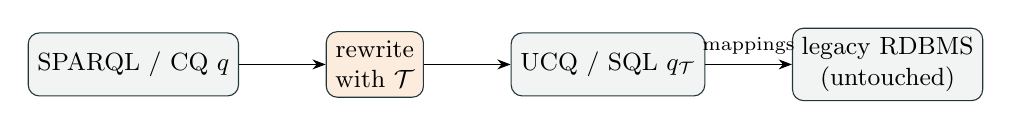
\begin{tikzpicture}[node distance=1.6cm, every node/.style={font=\small},
      box/.style={draw=ink, rounded corners, fill=ink!6, minimum height=0.8cm, align=center}]
    \node[box] (q) {SPARQL / CQ $q$};
    \node[box, right=1.1cm of q, fill=accent!15] (rw) {rewrite\\with $\mathcal{T}$};
    \node[box, right=1.1cm of rw] (sql) {UCQ / SQL $q_{\mathcal{T}}$};
    \node[box, right=1.1cm of sql] (db) {legacy RDBMS\\(untouched)};
    \draw[-{Stealth}] (q) -- (rw);
    \draw[-{Stealth}] (rw) -- (sql);
    \draw[-{Stealth}] (sql) -- node[above]{\scriptsize mappings} (db);
  \end{tikzpicture}
  \end{center}
  \begin{itemize}
    \item Ontology compiled into the \emph{query}, never into the data
      $\Rightarrow$ OBDA (Mastro, Ontop); the reason OWL~2~QL exists.
    \item Cost: the rewriting may grow exponentially in the size of the \emph{query}
      (not of the data) $\Rightarrow$ heavy optimisation and pruning in practice.
  \end{itemize}
\end{frame}

%%%%%%%%%%%%%%%%%%%%%%%%%%%%%%%%%%%%%%%%%%%%%%%%%%%%%%%%%%%%%%%%%%%%%%%%%%%%%%%
\section{Named DLs and OWL}

\begin{frame}{Named DLs and their OWL counterparts}
  \centering
  \begin{tabular}{@{}lll@{}}
    \toprule
    \textbf{Description Logic} & \textbf{OWL language} & \textbf{Complexity (concept sat.)}\\
    \midrule
    $\EL$ / $\EL^{++}$          & OWL~2~EL    & PTime-complete\\
    $\dllite{\mathcal{R}}$      & OWL~2~QL    & NLogSpace; $AC^0$ data compl.\ for CQs\\
    \dl{DLP} / $pD^*$-style     & OWL~2~RL    & PTime-complete\\
    $\ALC$                      & ---         & ExpTime-complete\\
    $\SHIF^{(\mathcal{D})}$     & OWL~1~Lite  & ExpTime-complete\\
    $\SHOIN^{(\mathcal{D})}$    & OWL~1~DL    & NExpTime-complete\\
    $\SROIQ^{(\mathcal{D})}$    & OWL~2~DL    & N2ExpTime-complete\\
    unrestricted, RDF semantics & OWL~2~Full  & undecidable\\
    \bottomrule
  \end{tabular}
  \vspace{1em}
  \begin{alertblock}{OWL Lite was not ``lite''}
    It is $\SHIF^{(\mathcal{D})}$: same worst-case complexity as $\SHIF$, and most of OWL~DL
    can be encoded into it --- hence effectively abandoned in OWL~2.
  \end{alertblock}
\end{frame}

%%%%%%%%%%%%%%%%%%%%%%%%%%%%%%%%%%%%%%%%%%%%%%%%%%%%%%%%%%%%%%%%%%%%%%%%%%%%%%%
\section{The three OWL 2 profiles}

\begin{frame}{Three profiles, three targets --- pairwise incomparable}
  \begin{columns}[T]
    \begin{column}{0.32\textwidth}
      \begin{block}{OWL 2 EL \ ($\EL^{++}$)}
        \footnotesize
        \textbf{Target:} very large terminologies (SNOMED~CT, GO, NCIt).\\[3pt]
        \textbf{Keeps:} $\sqcap$, $\exists R.C$, nominals, chains, $\mathsf{Self}$,
        domain/range, keys, datatypes.\\[3pt]
        \textbf{Drops:} $\forall$, $\sqcup$, $\neg$, inverses, cardinality,
        functional properties.\\[3pt]
        Classification is \hl{polynomial}.
      \end{block}
    \end{column}
    \begin{column}{0.32\textwidth}
      \begin{block}{OWL 2 QL \ ($\dllite{\mathcal{R}}$)}
        \footnotesize
        \textbf{Target:} query answering over RDBMS via rewriting (OBDA, Ontop).\\[3pt]
        \textbf{Left:} class or $\exists R.\top$; \textbf{right:} class, $\exists R.C$, $\neg$.\\[3pt]
        \textbf{Drops:} $\sqcup$, chains, functional \& transitive props, nominals, keys.\\[3pt]
        \hl{$AC^0$} data complexity.
      \end{block}
    \end{column}
    \begin{column}{0.32\textwidth}
      \begin{block}{OWL 2 RL}
        \footnotesize
        \textbf{Target:} rule engines, forward chaining over RDF (Datalog).\\[3pt]
        \textbf{Left:} $\sqcap$, $\sqcup$, $\exists R.C$, nominals; \textbf{right:} $\sqcap$,
        $\forall R.C$, ${\leq}1$, ${\leq}0$, $\neg$.\\[3pt]
        \textbf{No existential} on the right $\Rightarrow$ no blank-node generation.\\[3pt]
        \hl{PTime}; degrades gracefully on OWL~Full graphs.
      \end{block}
    \end{column}
  \end{columns}
\end{frame}

\begin{frame}{Profile comparison}
  \centering\footnotesize
  \begin{tabular}{@{}lccc@{}}
    \toprule
    \textbf{Construct} & \textbf{EL} & \textbf{QL} & \textbf{RL}\\
    \midrule
    $C \sqcap D$                & \tyes & partial & \tyes\\
    $C \sqcup D$                & \tno  & \tno    & subclass pos.\ only\\
    $\neg C$                    & \tno  & superclass pos.\ only & superclass pos.\ only\\
    $\exists R.C$               & \tyes & superclass pos.\ only & subclass pos.\ only\\
    $\forall R.C$               & \tno  & \tno    & superclass pos.\ only\\
    Nominals $\{a\}$            & \tyes & \tno    & \tyes\\
    Inverse roles $\inv{R}$     & \tno  & \tyes   & \tyes\\
    Cardinality restrictions    & \tno  & \tno    & ${\leq}1$, ${\leq}0$ only\\
    Functional properties       & \tno  & \tno    & \tyes\\
    Transitive properties       & \tyes & \tno    & \tyes\\
    Property chains             & \tyes & \tno    & \tyes\\
    $\exists R.\mathsf{Self}$   & \tyes & \tno    & \tno\\
    Keys                        & \tyes & \tno    & \tyes\\
    \midrule
    Data complexity             & PTime & $AC^0$  & PTime\\
    \bottomrule
  \end{tabular}
\end{frame}

%%%%%%%%%%%%%%%%%%%%%%%%%%%%%%%%%%%%%%%%%%%%%%%%%%%%%%%%%%%%%%%%%%%%%%%%%%%%%%%
\section{Rule-based entailment: the GraphDB rulesets}

\begin{frame}{Triple stores reason with rules, not DL reasoners}
  GraphDB rulesets: \texttt{empty}, \texttt{rdfs}, \texttt{rdfsplus},
  \texttt{owl-horst}, \texttt{owl-max}, \texttt{owl2-ql}, \texttt{owl2-rl}
  (+ \texttt{-optimized} variants).\\[4pt]
  The names suggest a mapping to the languages above --- \hl{but it is loose}:
  \begin{enumerate}
    \item \textbf{Rule engine.} Horn rules (\texttt{.pie}), forward chaining,
      closure fully materialised at load time.
    \item \textbf{RDF-based semantics.} Rules match triples, not axioms; classes may be
      instances; no Direct Semantics.
    \item \textbf{No syntactic check.} Any graph is accepted, in-profile or not.
  \end{enumerate}
  \begin{alertblock}{Consequence}
    No ruleset implements a full DL. Each is a \emph{Horn fragment} of some DL:
    sound, but incomplete w.r.t.\ the logic whose vocabulary it accepts.
  \end{alertblock}
\end{frame}

\begin{frame}{Mapping rulesets to DL families}
  \centering\scriptsize
  \begin{tabular}{@{}llp{7.2cm}@{}}
    \toprule
    \textbf{Ruleset} & \textbf{Closest DL / profile} & \textbf{DL axioms covered}\\
    \midrule
    \texttt{rdfs} & $\rho$df $\subset \dllite{\mathcal{R}}$
      & $A \sub B$, $P \sub Q$, $\exists P \sub A$ (domain), $\exists \inv{P} \sub A$ (range)\\
    \texttt{rdfsplus} & Horn-\dl{SHI} ($\approx$ DLP)
      & $+$ $P \eqv \inv{Q}$, $P \eqv \inv{P}$ (symmetry), $\mathsf{Trans}(P)$\\
    \texttt{owl-horst} & $pD^*$ $\approx$ Horn-\dl{SHOIF}
      & $+$ $a \approx b$, $\mathsf{Func}(P)$, $\mathsf{Func}(\inv{P})$,
        $\exists P.C \sub A$, $A \sub \forall P.C$, $A \eqv \exists P.\{o\}$, $A \eqv B$\\
    \texttt{owl-max} & Horn-$\SHIF^{(\mathcal{D})}$ (OWL Lite syntax)
      & $+$ $B \sqcup C \sub A$, intersections, ${\leq}1\,P$\\
    \texttt{owl2-rl} & OWL~2~RL $\subset$ Horn-$\SROIQ^{(\mathcal{D})}$
      & $+$ property chains, keys, disjoint properties, qualified ${\leq}1$\\
    \texttt{owl2-ql} & OWL~2~QL $\approx \dllite{\mathcal{R}}$
      & $A \sub B$, $A \sub \exists P.B$, role inclusions, inverses, disjointness\\
    \bottomrule
  \end{tabular}
  \vspace{1em}

  \raggedright\small
  Reference points: $\SHIF^{(\mathcal{D})}$ = OWL Lite, $\SHOIN^{(\mathcal{D})}$ = OWL~1~DL,
  $\SROIQ^{(\mathcal{D})}$ = OWL~2~DL. \hl{No ruleset for OWL~2~EL.}
\end{frame}

\begin{frame}{Why every ruleset is a Horn fragment}
  \begin{columns}[T]
    \begin{column}{0.48\textwidth}
      \begin{block}{No disjunctive consequences}
        \small
        A rule derives $A(a)$, never $A(a) \lor B(a)$.\\[4pt]
        $\cn{Staff} \eqv \cn{Academic} \sqcup \cn{TechnicalStaff}$\\[2pt]
        only $\cn{Academic} \sub \cn{Staff}$ is usable; the converse
        (tableau case analysis) is lost.
      \end{block}
    \end{column}
    \begin{column}{0.48\textwidth}
      \begin{block}{No new individuals}
        \small
        Rules never invent a witness.\\[4pt]
        $A \sub \exists P.B$ is accepted and stored,\\[2pt]
        but yields no $P$-successor --- nor anything that would follow from one.
      \end{block}
    \end{column}
  \end{columns}
  \vspace{1em}
  \small
  Together these two limitations account for most of the distance from the full logics.
\end{frame}

\begin{frame}{Ruleset by ruleset}
  \small
  \begin{description}[RDFS-Plus]
    \item[RDFS] Not a DL (metamodelling). DL-part $\subset \dllite{\mathcal{R}} \cap \EL$.
    \item[RDFS-Plus] Role axioms of \dl{SHI} (inverse, transitive) on top of the
      hierarchy; no new concept constructors. Within DLP (Grosof et al., WWW~2003).
    \item[OWL-Horst] Ter Horst's $pD^*$ (\emph{JWS}~2005): ``if''-semantics over RDFS.
      $\approx$ Horn-\dl{SHOIF}; sound, incomplete for \SHOIN. GraphDB goes beyond textbook
      $pD^*$ on \texttt{intersectionOf}.
    \item[OWL-Max] OWL Lite syntax, Horn consequences only. Adds subclass-side
      \texttt{unionOf}, ${\leq}1$ $\to$ \texttt{sameAs}, more consistency checks.
      Exact diff: compare the \texttt{.pie} files.
    \item[OWL 2 RL] Derived from DLP and $pD^*$. Sound \& complete for ground atoms
      \emph{on in-profile ontologies} (Thm.~PR1); sound but incomplete outside.
    \item[OWL 2 QL] GraphDB \emph{materialises} instead of rewriting --- forgoes the
      profile's main benefit; more permissive than the profile.
  \end{description}
  \vspace{2pt}
  \footnotesize\textbf{\texttt{-optimized}}: drops axiomatic triples and \texttt{rdfs:Resource}
  conclusions (+ a few more). The documented list does \emph{not} include domain/range.
\end{frame}

\begin{frame}[fragile]{Empirical check: set-up}
  \begin{itemize}
    \item Small university KG, one construct per axiom block.
    \item Five repositories: \texttt{rdfsplus}, \texttt{owl-horst}, \texttt{owl-max},
      \texttt{owl2-ql}, \texttt{owl2-rl} (all \texttt{-optimized}, \texttt{owl:sameAs} on).
    \item Two runs; Horst replaced by RL in the second; all else identical.
  \end{itemize}
  \vspace{0.5em}
  \begin{block}{The key trick: an individual with no asserted type}
\begin{lstlisting}
ex:teaches a owl:ObjectProperty ;
           rdfs:domain ex:Academic ; rdfs:range ex:Course .
ex:alice   ex:teaches ex:kg101 .     # no rdf:type for ex:alice
\end{lstlisting}
    \small Every class membership of \texttt{ex:alice} must be \emph{inferred}.
  \end{block}
\end{frame}

\begin{frame}{Empirical check: results}
  \centering\scriptsize
  \begin{tabular}{@{}llccccc@{}}
    \toprule
    & \textbf{Construct tested} & \textbf{RDFS+} & \textbf{Horst}$^{e}$ &
      \textbf{Max} & \textbf{QL} & \textbf{RL}\\
    \midrule
    Q1 & domain, subclass                        & \tno$^{a}$ & \tyes & \tyes & \tyes & \tyes\\
    Q2 & subproperty, range                      & \tno$^{a}$ & \tyes & \tyes & \tyes & \tyes\\
    Q3 & inverse, symmetric                      & \tyes & \tyes & \tyes & \tyes & \tyes\\
    Q3 & transitive                              & \tyes & \tyes & \tyes & \tno  & \tyes\\
    Q4 & equivalent class / property             & --$^{b}$ & \tyes & \tyes & \tyes & \tyes\\
    Q5 & sameAs via (inverse-)functional prop.   & \tno & \tyes & \tyes & \tno & \tyes\\
    Q6 & hasValue, some/allValuesFrom            & \tno & \tyes & \tyes & \tno & \tyes$^{f}$\\
    Q7 & intersection, subclass side             & \tno & \tyes$^{c}$ & \tyes & \tyes$^{d}$ & \tyes\\
    Q7 & intersection, superclass side           & \tno & \tyes & \tyes & \tyes & \tyes\\
    Q7 & union, subclass side                    & \tno & \tno & \tyes & \tno & \tyes\\
    Q8 & property chain                          & \tno & \tno & \tno & \tno & \tyes\\
    Q9 & keys                                    & \tno & \tno & \tno & \tno & \tyes\\
    \midrule
    Q10 & implicit triples                       & 193 & 337 & 361 & \textbf{1596} & \textbf{1263}\\
    \bottomrule
  \end{tabular}

  \vspace{4pt}
  \raggedright\tiny
  $^{a}$ unexpected. \ $^{b}$ not observable (depends on domain). \
  $^{c}$ beyond textbook $pD^*$. \ $^{d}$ beyond OWL~2~QL profile. \
  $^{e}$ first run only. \ $^{f}$ includes a classification the RL profile does not license.

  \vspace{4pt}\small
  On this test bed: \texttt{owl2-rl} $\supset$ \texttt{owl-max} $\supset$ \texttt{owl-horst}
  --- though not nested by design. \hl{RL is the only regime that passes every test.}
\end{frame}

\begin{frame}{Five deviations from expectations}
  \small
  \begin{enumerate}
    \item \textbf{\texttt{rdfsplus-optimized} applies neither domain nor range.}
      Inverse/symmetric/transitive work, so the ruleset is active; same symptom seen on RDFS.
      Not explained by the docs; \texttt{owl2-rl-optimized} is fine.
      \emph{To confirm on the non-optimised ruleset.}
    \item \textbf{OWL-Horst handles intersection in both directions} --- textbook $pD^*$ does not.
    \item \textbf{OWL~2~QL derives membership in an intersection} --- a subclass-side use
      $\dllite{\mathcal{R}}$ does not allow.
    \item \textbf{OWL~2~RL classifies beyond its profile.}
      $\cn{Supervisor} \eqv \exists\rn{supervises}.\cn{PhDStudent}$ is out of profile,
      yet \texttt{ex:alice} is typed as a supervisor.
      \emph{The profile restricts what is guaranteed, not what fires.}
    \item \textbf{OWL~2 rulesets materialise far more} (QL 1596, RL 1263 vs.\ 193--361):
      both type everything as \texttt{owl:Thing}; QL > RL despite being weaker.
  \end{enumerate}
\end{frame}

\begin{frame}{Practical consequences}
  \begin{itemize}
    \item \textbf{Names are not guarantees.} Weaker than the name (RDFS-Plus) or stronger
      than the profile (Horst, QL). \hl{Test the constructs you rely on.}
    \item \textbf{DL-illegal input is silently accepted.} \texttt{InverseFunctionalProperty}
      on a datatype property is outside \SHOIN/\SROIQ, yet yields \texttt{owl:sameAs}.
    \item \textbf{The gap to a DL reasoner is measurable.} Compare inferred class assertions
      with HermiT / Konclude (or ELK for the EL part).
    \item \textbf{Materialisation cost is not monotone in expressivity.} QL > RL $\gg$ Max.
    \item \textbf{Beyond RDFS-Plus, OWL~2~RL is the safe default} --- only regime passing every
      test, only one with chains and keys.
  \end{itemize}
\end{frame}

%%%%%%%%%%%%%%%%%%%%%%%%%%%%%%%%%%%%%%%%%%%%%%%%%%%%%%%%%%%%%%%%%%%%%%%%%%%%%%%
\section{Case study: ECMO 0.3.0}

\begin{frame}{ECMO 0.3.0 against the GraphDB rulesets}
  \begin{itemize}
    \item JRC ontology network for \textbf{emergency and crisis management}.
    \item Built on the \textbf{Sendai Framework} terminology; aligned to
      \textbf{DOLCE+DnS Ultralite} (DUL) through d0.
    \item Assessed modules: hub, core, core pattern, foundation, disaster, risk.
    \item Other domain modules and the inferred-axioms file not inspected
      $\Rightarrow$ \emph{indicative, not a complete profile}.
  \end{itemize}
  \vspace{0.5em}
  \begin{block}{The defined class carrying most semantic weight}
    \[
      \cn{Disaster} \eqv \cn{HazardousEvent} \sqcap
      \exists \rn{hasImpact}.(\cn{Impact} \sqcap
      \exists \rn{hasImpactIntensity}.\{\ind{VeryHighImpactIntensity}\})
    \]
    \small Only the right-to-left ($\sqsupseteq$) half is rule-expressible --- and only
    OWL~2~RL guarantees it. It lets a store classify a hazardous event as a disaster
    from its reported impacts.
  \end{block}
\end{frame}

\begin{frame}{ECMO constructs and ruleset support}
  \centering\scriptsize
  \setlength{\tabcolsep}{2.6pt}
  \renewcommand{\arraystretch}{0.95}
  \begin{tabular}{@{}p{3.0cm}p{6.3cm}cccccc@{}}
    \toprule
    \textbf{Construct} & \textbf{Example in ECMO} & \textbf{RDFS} & \textbf{RDFS+} &
      \textbf{Horst} & \textbf{Max} & \textbf{QL} & \textbf{RL}\\
    \midrule
    RDFS core & subclass, subproperty, domain, range
      & \tyes & \tyes & \tyes & \tyes & \tyes & \tyes\\
    Inverse properties & dozens of pairs, e.g.\ \texttt{hasHazardDeterminant}
      & & \tyes & \tyes & \tyes & \tyes & \tyes\\
    Transitive properties & \texttt{subsumedUnder}, \texttt{specializes}, \texttt{includesEvent}
      & & \tyes & \tyes & \tyes & \tno & \tyes\\
    Symmetric property & \texttt{isComplementaryTo}
      & & \tyes & \tyes & \tyes & \tyes & \tyes\\
    \texttt{hasValue}, superclass side
      & $\cn{DirectlyAffectedPopulation} \sub$\newline\hspace*{1em}$\exists\rn{hasAffectednessType}.\{\ind{Direct}\}$
      & & & \tyes & \tyes & \tno & \tyes\\
    \texttt{owl:sameAs} & the HIPS hazard individuals
      & & & \tyes & \tyes & \tno & \tyes\\
    Defined class & $\cn{Disaster}$ ($\sqcap$, nested $\exists$, \texttt{hasValue})
      & & & partial & partial & \tno & \tyes$^{a}$\\
    Union, subclass side & $\cn{Eventuality} \eqv \cn{Event} \sqcup \cn{EventType} \sqcup \cn{Situation}$
      & & & \tno & \tyes & \tno & \tyes\\
    Union, superclass side & $\cn{Assessment} \sub \cn{Eventuality} \sqcup \cn{InformationEntity}$
      & \tno & \tno & \tno & \tno & \tno & \tno\\
    $\exists$, superclass side & $\cn{Risk} \sub \exists\rn{hasHazardDeterminant}.\cn{Hazard}$
      & \multicolumn{6}{c}{no witness generated}\\
    Qualified cardinality & $\cn{Assessment} \sub {\geq}1\,\rn{assesses}.\cn{Entity}$
      & \tno & \tno & \tno & \tno & \tno & \tno\\
    Property chains & $\rn{isSettingFor} \circ \rn{isAbout} \sub \rn{assesses}$
      & & & & & \tno & \tyes\\
    Disjointness & \texttt{Frequent}/\texttt{InfrequentDisaster};\newline DUL: $\cn{Description} \sqcap \cn{Situation} \sub \bot$
      & \multicolumn{6}{c}{checks only (Max, RL)}\\
    Punning & hazard, risk and disaster subtypes
      & \multicolumn{6}{c}{transparent to rules}\\
    \bottomrule
  \end{tabular}

  \vspace{3pt}\raggedright\scriptsize $^{a}$ classifying direction ($\sqsupseteq$) only.
\end{frame}

\begin{frame}[fragile]{ECMO's DL expressivity --- and one out-of-DL axiom}
  \small
  Nominals, inverse \& transitive roles, chains, qualified cardinality, superclass union,
  datatypes $\Rightarrow$ \hl{$\SROIQ^{(\mathcal{D})}$ = OWL~2~DL}, outside all three profiles.
  \vspace{0.5em}
  \begin{alertblock}{Strictly, one axiom leaves OWL~2~DL}
    \texttt{foundation:assesses} is defined by a property chain $\Rightarrow$ \emph{non-simple};
    OWL~2~DL forbids cardinality restrictions on non-simple roles.
\begin{lstlisting}
foundation:Assessment rdfs:subClassOf [ a owl:Restriction ;
    owl:minQualifiedCardinality "1"^^xsd:nonNegativeInteger ;
    owl:onClass dul:Entity ; owl:onProperty foundation:assesses ] .
\end{lstlisting}
  \end{alertblock}
  \begin{block}{Fix}
    ${\geq}1\,R.C \equiv \exists R.C$, and existentials \emph{are} allowed on non-simple roles:
    replace with \texttt{owl:someValuesFrom dul:Entity} --- same meaning, OWL~2~DL restored.
  \end{block}
\end{frame}

\begin{frame}{What each ruleset delivers for ECMO}
  \small
  \begin{description}[OWL 2 RL]
    \item[RDFS-Plus] \emph{Minimum useful regime}: DnS hierarchy via transitive
      \texttt{subsumedUnder}/\texttt{specializes}, named inverses, domain/range.
      Verify domain/range on the deployed ruleset (see anomaly).
    \item[OWL-Horst] $+$ \texttt{hasValue} classifications (affected population, risk
      profile); merges HIPS hazards via \texttt{sameAs}.
    \item[OWL-Max] $+$ union: every event/situation a \texttt{d0:Eventuality} (largely
      redundant with domain axioms).
    \item[OWL 2 RL] \hl{Only one} to fire the chains to DUL setting/aboutness, reliably
      classify \texttt{Disaster}, and check disjointness guards.
    \item[OWL 2 QL] \textcolor{nored}{Unsuitable}: no transitivity $\Rightarrow$ whole
      \texttt{subsumedUnder} hierarchy lost; no chains, no \texttt{hasValue}.
    \item[None] Superclass union, superclass existentials (four determinants of
      \texttt{Risk}, \texttt{Signal}, \texttt{EventValidation}), cardinality
      $\Rightarrow$ need a DL reasoner.
  \end{description}
\end{frame}

\begin{frame}[fragile]{ECMO deployment notes}
  \small
  \begin{itemize}
    \item \textbf{Imports are not followed.} Load all modules and DUL/d0 explicitly ---
      without DUL, chains have nothing to fire on and disjointness guards are absent.
    \item \textbf{Import closure incomplete as distributed.} \texttt{0.3.0-alignments/}
      missing; \texttt{frames} (imported by \texttt{ecmo-core}) has no catalog entry.
    \item \textbf{Recommended:} OWL~2~RL in the store $+$ offline DL reasoner (Konclude / HermiT)
      for non-Horn consequences. \texttt{ecmo-inferredaxioms.ttl} may already be that output
      (not verified).
    \item \textbf{Modelling point:} \texttt{risk:Risk} $\sub$ \texttt{hazard:Hazard} $\Rightarrow$
      every risk typed as a hazard --- at odds with risk as $f$(hazard, exposure, vulnerability,
      capacity).
  \end{itemize}
  \begin{block}{Full profile with ROBOT (once the catalog is fixed)}
\begin{lstlisting}[language={}]
robot merge --catalog catalog-v001.xml --input ecmo-core.ttl --output merged.owl
robot validate-profile --profile RL --input merged.owl --output rl-violations.txt
robot validate-profile --profile DL --input merged.owl --output dl-violations.txt
\end{lstlisting}
  \end{block}
\end{frame}

%%%%%%%%%%%%%%%%%%%%%%%%%%%%%%%%%%%%%%%%%%%%%%%%%%%%%%%%%%%%%%%%%%%%%%%%%%%%%%%
\section{Openly available reasoners}

\begin{frame}{Three warnings before the tables}
  \begin{enumerate}
    \item \textbf{``Supports \dl{X}'' is a claim about the calculus, not the code.}
      Gaps usually in datatypes, nominals, exotic role axioms.
    \item \textbf{Maintenance, not expressivity, is the binding constraint.}
      A 2023 review: fewer than half of reasoners active in the previous three years;
      HermiT among the effectively abandoned (Abicht, arXiv:2309.06888).
    \item \textbf{The comparative evidence is dated.} Last OWL Reasoner Evaluation:
      ORE~2015 (Parsia et al., \emph{JAR}~2017). No common benchmark since.
  \end{enumerate}
\end{frame}

\begin{frame}{OWL 2 DL: the $\SROIQ$ tier}
  \centering\scriptsize
  \begin{tabular}{@{}lllp{7.2cm}@{}}
    \toprule
    \textbf{Reasoner} & \textbf{Expressivity} & \textbf{Method} & \textbf{Notes}\\
    \midrule
    \rowcolor{accent!12}
    Konclude & $\SROIQ\mathcal{V}^{(\mathcal{D})}$ & tableau + saturation
      & C++, LGPLv3. $\mathcal{V}$ = nominal schemas. Won most DL tracks of ORE~2015\\
    \rowcolor{accent!12}
    HermiT & $\SROIQ^{(\mathcal{D})}$ & hypertableau
      & Java. Upstream dead since 1.3.8; OWL~API fork unsupported. Ships with Prot\'eg\'e\\
    FaCT++ & $\SROIQ^{(\mathcal{D})}$ & optimised tableau & C++. Last commit 2017; ships with Prot\'eg\'e\\
    JFact & $\SROIQ^{(\mathcal{D})}$ & tableau & Java port of FaCT++, under OWL~API umbrella\\
    Openllet & $\SROIQ^{(\mathcal{D})}$ & tableau & Community fork of Pellet; sporadic updates\\
    Pellet & $\SROIQ^{(\mathcal{D})}$ & tableau & Abandoned; use Openllet\\
    Sequoia & $\dl{SRIQ}$ & consequence-based & Scala. No nominals --- traded for scalability\\
    Racer & $\dl{SRIQ}^{(\mathcal{D})}$ & tableau & Common Lisp, BSD-3. Abandoned\\
    Vampire & FOL & superposition & General prover; OWL~DL by translation\\
    \bottomrule
  \end{tabular}
  \vspace{0.6em}

  \raggedright\small
  Realistic choices: \hl{Konclude} (fastest, actively developed) or \hl{HermiT}
  (OWL~API-native, ubiquitous, unmaintained).
\end{frame}

\begin{frame}{OWL 2 EL and OWL 2 QL tiers}
  \centering\scriptsize
  \begin{tabular}{@{}lllp{6.8cm}@{}}
    \toprule
    \multicolumn{4}{@{}l}{\textbf{EL tier}}\\
    \midrule
    \rowcolor{accent!12}
    ELK & $\EL^{++}$, safe nominals & concurrent cons.-based
      & Java, Apache~2.0. Partial $\neg$, $\sqcup$, datatypes; incremental. De-facto
        biomedical standard; warns on unsupported constructs\\
    jcel & $\EL^{+}$ & completion rules & Java. Prot\'eg\'e plugin\\
    CEL & $\EL^{+}$ & completion rules & Original large-scale EL reasoner; historical\\
    ElepHant & $\EL^{+}$ & cons.-based & C. Small memory/CPU, embedded use\\
    Whelk & $\EL$ + RL & cons.-based & Scala. EL TBox + RL ABox; in ROBOT / OBO toolchain\\
    Snorocket & EL subset & completion rules & Java. Concrete domains; SNOMED~CT tooling\\
    \midrule
    \multicolumn{4}{@{}l}{\textbf{QL tier (rewriting / OBDA)}}\\
    \midrule
    \rowcolor{accent!12}
    Ontop & $\dllite{\mathcal{R}}$ + RDFS & rewriting to SQL
      & Java, Apache~2.0, active (5.5.0, Feb.~2026). SPARQL over VKGs via R2RML\\
    Mastro & $\dllite{\mathcal{A}}$ & rewriting to SQL & Sapienza. Academic licence, not open source\\
    Clipper & Horn-$\dl{SHIQ}$ & to Datalog & Abandoned; DLV back end no longer distributed\\
    Requiem & $\dl{ELHIO}$ & resolution & Prototype; not maintained\\
    \bottomrule
  \end{tabular}
  \vspace{0.5em}

  \raggedright\small
  QL is effectively single-vendor: \hl{Ontop} is the only open, maintained rewriting system.
\end{frame}

\begin{frame}{OWL 2 RL: rules and materialisation}
  \centering\scriptsize
  \begin{tabular}{@{}lllp{6.0cm}@{}}
    \toprule
    \textbf{Reasoner} & \textbf{Expressivity} & \textbf{Method} & \textbf{Notes}\\
    \midrule
    RDFox & OWL~2~RL, Datalog, SWRL & parallel materialisation
      & C++. Fastest in class; commercial, free academic licences\\
    VLog & Datalog + existential rules & chase & Open source; OWL~RL via axiom-to-rule translation\\
    OWL-RL & OWL~2~RL & forward chaining & Python on RDFLib. Convenient, not fast\\
    reasonable & OWL~2~RL subset & forward chaining & Rust + Python bindings; much faster than OWL-RL\\
    Arachne & OWL~RL & Rete & Scala. Built for GO causal activity models\\
    Apache Jena & RDFS, partial OWL & fwd/bwd rules & Deliberately incomplete; ubiquitous\\
    GraphDB & RDFS $\to$ OWL~2~RL/QL & forward chaining
      & Commercial + free edition. Horn fragments; names $\neq$ guarantees\\
    EYE & N3 rules & Euler-path chaining & Prolog/Wasm, very active; OWL-adjacent rules\\
    \bottomrule
  \end{tabular}
  \vspace{0.6em}

  \raggedright
  \textbf{Hybrid / pay-as-you-go}\\[2pt]
  \small
  \textbf{PAGOdA}: RDFox for the RL bulk, HermiT for the hard residue. \;
  \textbf{MORe}, \textbf{Chainsaw}: modular routing ELK/HermiT (unmaintained). \;
  \textbf{TrOWL}: approximate DL into QL/EL.
\end{frame}

\begin{frame}{Choosing a reasoner}
  \small
  Expressivity narrows the field; the remaining criteria usually decide it.
  \vspace{0.5em}

  \centering
  \begin{tabular}{@{}p{5.6cm}p{6.8cm}@{}}
    \toprule
    \textbf{Scenario} & \textbf{Choice}\\
    \midrule
    Large terminology, EL-shaped & \textbf{ELK} --- unmatched at SNOMED scale; incremental mode\\
    Full OWL~2~DL, performance matters & \textbf{Konclude}; pure Java/OWL~API $\to$ HermiT (unmaintained)\\
    Data in an RDBMS, ontology as query interface & \textbf{Ontop}\\
    Large RDF graphs, forward chaining OK & \textbf{RDFox} if licence OK; else VLog, Arachne, or the store's own\\
    Embedded / constrained hardware & \textbf{ElepHant} (EL) or \textbf{LiRoT} (RL subset)\\
    \bottomrule
  \end{tabular}
\end{frame}

%%%%%%%%%%%%%%%%%%%%%%%%%%%%%%%%%%%%%%%%%%%%%%%%%%%%%%%%%%%%%%%%%%%%%%%%%%%%%%%
\begin{frame}{Take-aways}
  \begin{enumerate}
    \item DL names are \textbf{compositional}; \dlliteplain{} is the exception ---
      designed bottom-up for \textbf{FOL-rewritability}.
    \item The OWL~2 profiles are \textbf{pairwise incomparable}: EL for big TBoxes,
      QL for OBDA, RL for rules over RDF.
    \item Triple-store rulesets are \textbf{Horn fragments} under RDF semantics:
      no disjunction, no witnesses, no syntactic check.
    \item \textbf{Names are not guarantees} --- RDFS-Plus under-delivers, Horst/QL/RL
      over-deliver. Test what you rely on.
    \item For \textbf{ECMO}: OWL~2~RL in the store + an offline DL reasoner; fix the
      cardinality-on-non-simple-role axiom and the import catalog.
    \item Among reasoners, \textbf{maintenance} decides: Konclude, ELK, Ontop are the
      living references of their tiers.
  \end{enumerate}
\end{frame}

\end{document}
